% Template for Elsevier CRC journal article
% version 1.2 dated 08 January 2015

% This file (c) 2009-15 Elsevier Ltd.  Modifications may be freely made,
% provided the edited file is saved under a different name

% This file contains modifications for Nuclear and Particle Physics Proceedings

% Changes since version 1.0
% - elsarticle class option changed from 1p to 3p (to better reflect CRC layout)
%
% version 1.2
% - Journal name changed to "Nuclear and Particle Physics Proceedings"

%-----------------------------------------------------------------------------------

%% This template uses the elsarticle.cls document class and the extension package ecrc.sty
%% For full documentation on usage of elsarticle.cls, consult the documentation "elsdoc.pdf"
%% Further resources available at http://www.elsevier.com/latex

%-----------------------------------------------------------------------------------

%%%%%%%%%%%%%%%%%%%%%%%%%%%%%%%%%%%%%%%%%%%%%%
%%%%%%%%%%%%%%%%%%%%%%%%%%%%%%%%%%%%%%%%%%%%%%
%%                                          %%
%% Important note on usage                  %%
%% -----------------------                  %%
%% This file must be compiled with PDFLaTeX %%
%% Using standard LaTeX will not work!      %%
%%                                          %%
%%%%%%%%%%%%%%%%%%%%%%%%%%%%%%%%%%%%%%%%%%%%%%
%%%%%%%%%%%%%%%%%%%%%%%%%%%%%%%%%%%%%%%%%%%%%%

%-------NEW COMMANDS------------
\newcommand{\trento}{T\raisebox{-0.5ex}{R}ENTo}

%-------pic folder--------------



%% The '3p' and 'times' class options of elsarticle are used for Elsevier CRC
\documentclass[3p,times,twocolumn]{elsarticle}

%% The `ecrc' package must be called to make the CRC functionality available
\usepackage{ecrc}
\graphicspath{{fig/}}
\usepackage{tabularx}
%% The ecrc package defines commands needed for running heads and logos.
%% For running heads, you can set the journal name, the volume, the starting page and the authors

%% set the volume if you know. Otherwise `00'
\volume{00}

%% set the starting page if not 1
\firstpage{1}

%% Give the name of the journal
\journalname{Nuclear and Particle Physics Proceedings}

%% Give the author list to appear in the running head
%% Example \runauth{C.V. Radhakrishnan et al.}
\runauth{}

%% The choice of journal logo is determined by the \jid and \jnltitlelogo commands.
%% A user-supplied logo with the name <\jid>logo.pdf will be inserted if present.
%% e.g. if \jid{yspmi} the system will look for a file yspmilogo.pdf
%% Otherwise the content of \jnltitlelogo will be set between horizontal lines as a default logo

%% Give the abbreviation of the Journal.
\jid{nppp}

%% Give a short journal name for the dummy logo (if needed)
\jnltitlelogo{Nuclear and Particle Physics Proceedings}

%% Hereafter the template follows `elsarticle'.
%% For more details see the existing template files elsarticle-template-harv.tex and elsarticle-template-num.tex.

%% Elsevier CRC generally uses a numbered reference style
%% For this, the conventions of elsarticle-template-num.tex should be followed (included below)
%% If using BibTeX, use the style file elsarticle-num.bst

%% End of ecrc-specific commands
%%%%%%%%%%%%%%%%%%%%%%%%%%%%%%%%%%%%%%%%%%%%%%%%%%%%%%%%%%%%%%%%%%%%%%%%%%

%% The amssymb package provides various useful mathematical symbols
\usepackage{amssymb}
%% The amsthm package provides extended theorem environments
%% \usepackage{amsthm}

%% The lineno packages adds line numbers. Start line numbering with
%% \begin{linenumbers}, end it with \end{linenumbers}. Or switch it on
%% for the whole article with \linenumbers after \end{frontmatter}.
%% \usepackage{lineno}

%% natbib.sty is loaded by default. However, natbib options can be
%% provided with \biboptions{...} command. Following options are
%% valid:

%%   round  -  round parentheses are used (default)
%%   square -  square brackets are used   [option]
%%   curly  -  curly braces are used      {option}
%%   angle  -  angle brackets are used    <option>
%%   semicolon  -  multiple citations separated by semi-colon
%%   colon  - same as semicolon, an earlier confusion
%%   comma  -  separated by comma
%%   numbers-  selects numerical citations
%%   super  -  numerical citations as superscripts
%%   sort   -  sorts multiple citations according to order in ref. list
%%   sort&compress   -  like sort, but also compresses numerical citations
%%   compress - compresses without sorting
%%
%% \biboptions{comma,round}

% \biboptions{}

% if you have landscape tables
\usepackage[figuresright]{rotating}

% put your own definitions here:
%   \newcommand{\cZ}{\cal{Z}}
%   \newtheorem{def}{Definition}[section]
%   ...

% add words to TeX's hyphenation exception list
%\hyphenation{author another created financial paper re-commend-ed Post-Script}

% declarations for front matter

\begin{document}

\begin{frontmatter}

%% Title, authors and addresses

%% use the tnoteref command within \title for footnotes;
%% use the tnotetext command for the associated footnote;
%% use the fnref command within \author or \address for footnotes;
%% use the fntext command for the associated footnote;
%% use the corref command within \author for corresponding author footnotes;
%% use the cortext command for the associated footnote;
%% use the ead command for the email address,
%% and the form \ead[url] for the home page:
%%
%% \title{Title\tnoteref{label1}}
%% \tnotetext[label1]{}
%% \author{Name\corref{cor1}\fnref{label2}}
%% \ead{email address}
%% \ead[url]{home page}
%% \fntext[label2]{}
%% \cortext[cor1]{}
%% \address{Address\fnref{label3}}
%% \fntext[label3]{}

\dochead{}
%% Use \dochead if there is an article header, e.g. \dochead{Short communication}

\title{Constaints on rapidity-dependent initial conditions from particle charged particle pseudorapidity densities and correlations at LHC}

%% use optional labels to link authors explicitly to addresses:
%% \author[label1,label2]{<author name>}
%% \address[label1]{<address>}
%% \address[label2]{<address>}

\author{Weiyao Ke}
\author{J. Scott Moreland}
\author{Jonah E. Bernhard}
\author{Steffen A. Bass}

\address{Department of Physics, Duke University, Durham, NC 27708-0305, United States}

\begin{abstract}
The initial three-dimensional entropy distribution of the quark-gluon plasma produced in relativistic heavy-ion collision is systematically studied using a parametric initial condition.
We apply a cumulant generating function approach to parametrize the rapidity dependence of local entropy deposition and extend the boost-invariant initial condition model \trento~to include longitudinal structure.
Two different parametrizations are tested and their parameters optimized by comparing to centrality dependent charged particle pseudorapidity densities of p+Pb (5.02A TeV) and Pb+Pb (2.76A TeV) using Bayesian inference.
Successful parametrizations are then selected based on their ability to describe two-particle psuedorapidity correlations.
Finally, we predict the pseudorapidity dependent flows and event-plane decorrelations using this optimized initial condition and a 3+1D hybrid hydro+micro model.

\end{abstract}

\begin{keyword}
initial condition \sep charged particle density \sep two-particle correlation
%% keywords here, in the form: keyword \sep keyword

%% MSC codes here, in the form: \MSC code \sep code
%% or \MSC[2008] code \sep code (2000 is the default)

\end{keyword}

\end{frontmatter}

%%
%% Start line numbering here if you want
%%
% \linenumbers

%% main text
\section{Introduction}
\label{Introduction}
Ultra-relativistic heavy-ion collisions produce a strongly coupled quark-gluon plasma (sQGP) whose dynamics are well described by models based on hydrodynamics.
A prerequisite for hydrodynamic modelign and also a major source of uncertainty  is the knowledge of initial condition which specifies the initial spatial entropy / energy distribution at the starting time of the hydrodynamic evolution.
Most current initial condition models assume longitudinal boost-invariance.
However, this assumption is explicitly broken in asymmetric collision systems such as p+Pb.
Even in central Pb+Pb collision, nucleon position fluctuations could introduce an intricate local longitudinal dependence, which can affect observable quantities as well as correlations between hard probes and soft particles.

Previous approaches for the development of the three-dimensional initial conditions utilized a number of different physical pictures, from MC Glauber extensions \cite{Bozek:2015bha}, minijet production and string formation \cite{Wang:1991hta} to most recently CGC effective field theory \cite{Schenke:2016ksl}.
In this work, we use a parametric initial condition which encodes different types of longitudinal entropy deposition schemes with tunable parameters.
Although our approach does not rely on a specific physical mechanism, the true value of a parametric model is its capability of generating initial condition compatible with experimental data and thus providing guidance to the different physical approaches of initial conditions.
%In fact, it is actually a non-trivial task to infer the local longitudinal dependence of the initial fireball from final state observables.
%The optimized 3D initial condition model benefits the study of longitudinal dynamics and rapidity dependent observables such as pseudorapidity dependent flows and event-plane decorrelations.

\section{Initial Condition Model}
\label{Model}
We extend the boost-invariant parametric initial condition model \trento~\cite{Moreland:2014oya} by introducing a local longitudinal structure based on a cumulant generating function approach.
The physics of \trento~is described in detail in reference \cite{Moreland:2014oya}. The main feature of \trento~is that it maps the nuclear participant densities $T_A(\vec{x}_{\perp})$ and $T_B(\vec{x}_{\perp})$ to a mid-rapidity entropy deposition in a flexible way controlled by a continuous parameter $p$.
Using Bayesian techniques, it has been shown that the calibrated \trento~initial condition together with the state-of-the-art dynamic modeling can explain annisotropic flows, particle yields and mean transverse momentum at mid-rapidity to an unprecedented level of accuracy \cite{Bernhard:2016tnd}, validating the effectiveness of \trento~at mid-rapidity.

The three dimensional extension proceed as  follows: 
Assuming that the longitudinal asymmetry of local entropy deposition is triggered by the imbalance between local projectile and target, we parametrize the fist three rapidity-cumulants of the local entropy distribution as functions of $T_A(\vec{x}_{\perp})$ and $T_B(\vec{x}_{\perp})$,
\begin{eqnarray}
\frac{ds(\vec{x}_{\perp}, \eta_s)}{dx_{\perp}^2 d\eta_s} \propto f(\vec{x}_{\perp})g(y; \mu(\vec{x}_{\perp}), \sigma(\vec{x}_{\perp}), \gamma(\vec{x}_{\perp}))\frac{dy}{d\eta}.
\end{eqnarray}
Here, $f(\vec{x}_{\perp})$ is the  mid-rapidity entropy density calculated from  \trento. The function $g(y; \mu, \sigma, \gamma)$ encodes the rapidity dependence,  its mean ($\mu$), standard deviation ($\sigma$) and skewness ($\gamma$) can also be functions of $T_A$ and $T_B$.
We tested two parametrization as shown in table \ref{tab:parametrization}.
In both cases, the mean of entropy distribution is proportional to the center-of-mass rapidity of the incoming nuclear densities and the standard deviation is independent of nuclear densities. 
The relative-skew model has a skewness proportional to the relative difference of $T_A$ and $T_B$, whereas the absolute-skew model uses the absolute difference between them.
The function $g(y)$ is then constructed from the inverse Fourier transformation of the cumulant-generating function
\begin{eqnarray}
g(y) &=& \mathcal{F}^{-1}\left\lbrace\tilde{g}(k)\right\rbrace \\
\tilde{g}(k) &=& \exp \left\lbrace i\mu k - \frac{1}{2}\sigma^2 k^2 - \frac{i}{6}\sigma^3 \gamma'k^3\right\rbrace
\end{eqnarray}
where $\gamma$ is replaced by $\gamma' = \gamma\exp(-\frac{1}{2}\sigma^2k^2)$ to regulate the behavior of the function at large values of rapidity.
Finally, the longitudinal profile $g(y)dy/d\eta$ is normalized by its value at $\eta=0$ so that the mid-rapidity behavior of \trento~remains unchanged.
Figure \ref{fig:trento} shows a sample Pb+Pb event and a sample p+Pb event generated from the \trento-3d model.

\begin{table}
  \caption{
    \label{tab:parametrization}
    Rapidity-dependent initial condition parametrizations with two different models for the skewness parameter. The constant $T_0 = 1$~fm$^{-2}$ preserves the desired dimensionality.
  }
  \begin{tabular}{cccc}
\hline\hline
      & \multicolumn{3}{c}{Distribution cumulant:} \\
      Model & \multicolumn{1}{c}{mean $\mu$} & \multicolumn{1}{c}{std.\ $\sigma$} & \multicolumn{1}{c}{skewness $\gamma$} \\
\hline
        Relative  & $\frac{1}{2} \mu_0 \log(T_A/T_B)$ & $\sigma_0$ & $\gamma_0 \frac{T_A - T_B}{T_A + T_B}$ \smallskip \\
        Absolute & $\frac{1}{2} \mu_0 \log(T_A/T_B)$  & $\sigma_0$ & $\gamma_0 (T_A - T_B)/T_0$ \\
\hline\hline
  \end{tabular}
\end{table}

\begin{figure}
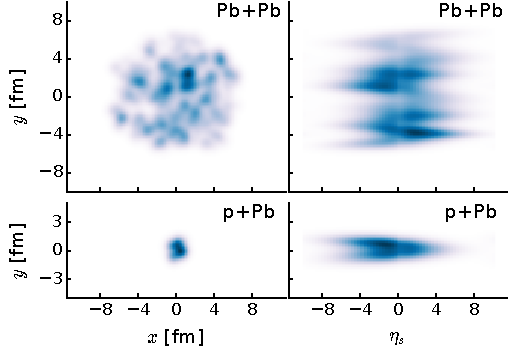
\includegraphics[width=\columnwidth]{trento3d_example.pdf}
\caption{\label{fig:trento} Initial entropy density in sample Pb+Pb (upper) and p+Pb (lower) events for cross sections of the $\eta=0$ and $x=0$ planes (left and right columns). The event is constructed using the relative-skew model.}
\end{figure}

\section{Model Calibration using Bayesian Statistics}
The original \trento~already has five parameters that control entropy deposition at midrapidity:
\begin{enumerate}
  \item[1--2.] two normalization factors for Pb+Pb and p+Pb collisions at $\sqrt{s}=2.76$~TeV and 5.02~TeV,
  \item[3.] the parameter $p$ which modulates midrapidity entropy deposition in \trento,
  \item[4.] a gamma shape parameter $k$, which controls the proton-proton multiplicity fluctuations,
  \item[5.] and a Gaussian nucleon width $w$, which determines initial the state granularity;
\end{enumerate}
The 3D extension introduces four more parameters to the model:
\begin{enumerate}
  \setcounter{enumi}{6}
  \item[6--8.] three coefficients which modulate the local rapidity distribution's shift $\mu_0$, width $\sigma_0$, and skewness $\gamma_0$,
  \item[9.] and a Jacobian factor $J$ for the conversion from rapidity to pseudorapidity.
\end{enumerate}

\begin{center}
\begin{figure*}
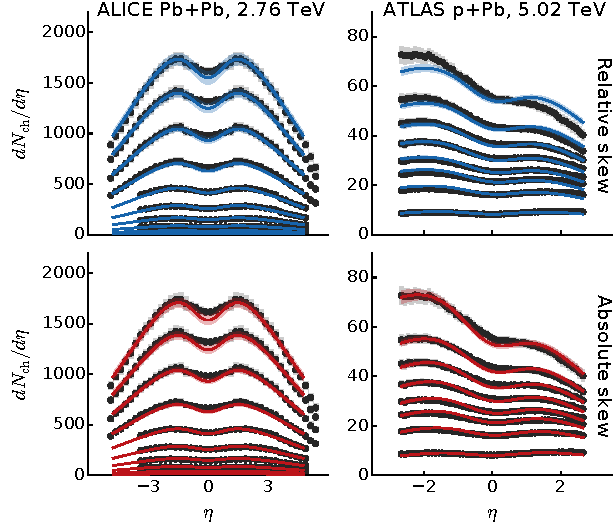
\includegraphics[scale=0.85]{chg_particle_rapidity.pdf}
\hfill
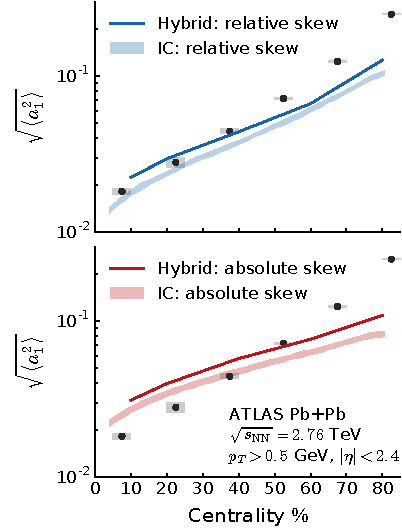
\includegraphics[scale=0.85]{fw_correlation_a1.pdf}
\caption{
	\label{fig:calibrate}
	Left: calibrated initial conditon models' mean prediction of $dN_{ch}/d\eta$ with uncertainty compared to ALICE (Pb+Pb) and ATLAS (p+Pb) data. Right: calibrated initial condition and hybrid model calculation ($\eta/s=0.2, \zeta/s=0$) of $\langle a_1^2\rangle^{1/2}$ compared to ATLAS data.
	}
\end{figure*}
\end{center}
To globally tune all parameters, we perform a Bayesian model-to-data comparison as described by \cite{Bernhard:2015hxa}.
Since the 3+1D hydrodynamic simulation is computationally expensive, we directly compare the initial condition calculation  to the charged particle densities assuming,
\begin{eqnarray}
\frac{ds}{d\eta_s} \sim \frac{dN_{ch}}{d\eta}.
\end{eqnarray}
Using Latin-hypercube sampling, we randomly sample 200 design parameter points from uniform distributions  over a reasonable range of the nine-dimensional parameter space. Then we generate $\mathcal{O}(10^4)$ initial condition events for each design point and calculate $dN_{ch}/d\eta$.
We train Gaussian emulators to interpolate between these design pointers and predict the outcomes at new parameters points.
The nine-dimensional posterior probability distribution of model parameters after comparing to experimental data can be calculated from Bayes theorem and explored via Markov Chain Monte Carlo (MCMC).

\begin{center}
\begin{figure*}
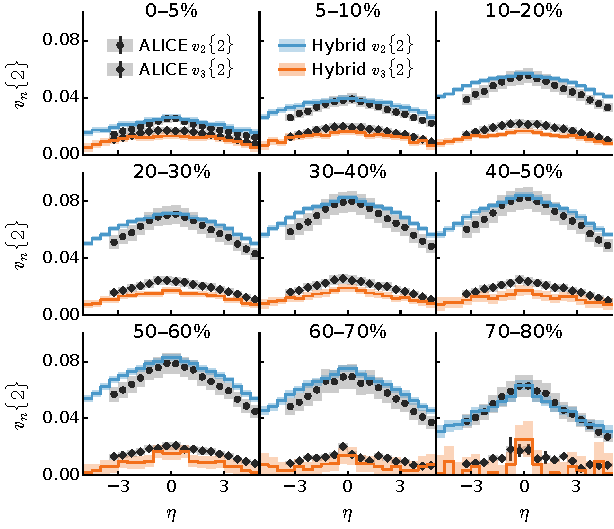
\includegraphics[scale=0.85]{vn_eta.pdf}
\hfill
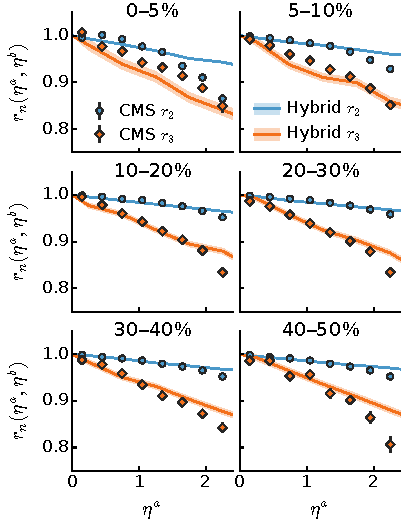
\includegraphics[scale=0.85]{evt_pln_decorr.pdf}
\caption{
	\label{fig:eta-obs}
	Left: Calibrated relative-skew model and hybrid model calculation ($\eta/s=0.3, \zeta/s=0$) of pseudorapidity dependent flows compared to ALICE data. Right: hybrid model calculation of event-plane decorrelation ($\eta/s=0.2, \zeta/s=0$) compared to CMS data.}
\end{figure*}
\end{center}
\section{Result}
\label{Result}
The performance of the calibrated models is visualized in the left panel of figure~\ref{fig:calibrate}, 100 parameter sets are sampled from each model's posterior distribution and the corresponding $dN_{ch}/d\eta$ are calculated.
Lines denote the posterior samples' average and thin bands their corresponding standard deviation and black data points are ALICE (Pb+Pb) \cite{Abbas:2013bpa, ALICE:2015kda} and ATLAS (p+Pb) \cite{Aad:2015zza} measurements.
This result shows that the calibrated models can simultaneously describe $dN_{ch}/d\eta$ of both p+Pb and Pb+Pb collision systems at different centralities, illustrating the flexibility of the generating function approach.

Using the highest likelihood parameter set from the posterior distribution, we perform a full model calculation with each initial condition setup, including a 3+1D hydrodynamic evolution \cite{Karpenko:2013wva} and hadronic rescattering \cite{Bass:1998ca, Bleicher:1999xi}.
Then, we extract the root-mean-square of two-particle pseudorapidity correlation coefficient $a_1$ defined in \cite{Bzdak:2012tp}, shown in the right panel of figure~\ref{fig:calibrate} for both relative-skew model and absolute-skew model along with ATLAS measurements \cite{ATLAS:2015kla}. 
The bands represent the initial condition and the lines the full hybrid model calculation.
One finds that although the absolute-skew model describes high-multiplicity p+Pb $dN_{ch}/d\eta$ a little better than the relative-skew mode, it completely fails to predict the correlation observable $\langle a_1^2\rangle^{1/2}$.
On the other hand the relative-skew model agrees with $dN_{ch}/d\eta$ data within $10\%$ and also describes the $\langle a_1^2\rangle^{1/2}$ upto $50\%$ centrality.
Therefore, we conclude that the relative-skew model is a better parametrization of the initial 3D entropy deposition. 

To further validate the calibrated relative-skew model, we use it to predict  pseudorapidty-dependent flow and event-plane decorrelations.
The left panel of figure \ref{fig:eta-obs}~shows the comparison of $v_2(\eta)$ and $v_3(\eta)$ to the recent ALICE measurement \cite{Adam:2016ows} at various centralities. We find generally good agreement with the data.
Note that the ALICE data is extrapolated to $p_T = 0~\textrm{GeV}$, we therefore used an unusual large $\eta/s=0.3$ in this calculation in order to compensate for the effect from over-predicting $\langle p_T\rangle$ with zero bulk viscosity.
In the right panel of figure \ref{fig:eta-obs}, the event-plane decorrelations quantified by the factorization ratio $r_2$ and $r_3$ are compared to previous CMS measurements \cite{Khachatryan:2015oea}.
Again, the relative-skew model combined with a 3+1D hybrid model well describes the data very well for all six centralities.

\section{Conclusion}
\label{Conclusion}
We have extended the parametric boost-invariant initial condition model \trento to include longitudinal degrees of freedom.
The mean, standard deviation and skewness of the local rapidity distribution is parametrized as function of nuclear participant densities.
Two different parametrizations, namely the relative-skew and absolute-skew model are proposed and calibrated using Bayesian inference with centrality dependent $dN_{ch}/d\eta$ data for both p+Pb and Pb+Pb collision systems.
The relative-skew model is favored since it can describe both single particle pseudo-rapidity distribution as well as two-particles pseudo-rapidity correlations for a wide range of centralities.
Combing the calibrated relative-skew initial condition and a 3+1D hybrid evolution model, the pseudo-rapidity dependent flow and event-plant decorrelation in Pb+Pb collision are predicted.
The fact that the model calibrated on transverse-integrated observables such as $dN_{ch}/d\eta$ and $\langle a_1^2\rangle^{1/2}$ can reproduce the flow and event-plane decorrelations, which are sensitive to the longitudinal evolution of the transverse structure, is a non-trivial result.
This simple model provides direct feedback for first-principal calculations of QGP initial condition and also benefits event-by-event study of 3+1D dynamics of relativistic heavy-ion collisions. 

Computational resources were provided by the Open Science Grid (OSG), which is supported by the U.S Department of Energy's Office of Science. This work has been supported by the U.S Department of Energy under grant DE-FG02-05ER41367 and the National Science Foundation under grant NSF-ACI-1550225.

%% The Appendices part is started with the command \appendix;
%% appendix sections are then done as normal sections
%% \appendix

%% \section{}
%% \label{}

%% References
%%
%% Following citation commands can be used in the body text:
%% Usage of \cite is as follows:
%%   \cite{key}         ==>>  [#]
%%   \cite[chap. 2]{key} ==>> [#, chap. 2]
%%

%% References with BibTeX database:
%%\nocite{*}
\bibliographystyle{elsarticle-num}
\bibliography{Weiyao_K}

%% Authors are advised to use a BibTeX database file for their reference list.
%% The provided style file elsarticle-num.bst formats references in the required Procedia style

%% For references without a BibTeX database:

% \begin{thebibliography}{00}

%% \bibitem must have the following form:
%%   \bibitem{key}...
%%

% \bibitem{}

% \end{thebibliography}

\end{document}

%%
%% End of file `nuphbp-template.tex'. 
